\documentclass{beamer}
\usetheme{CambridgeUS}
\usecolortheme{dolphin}
%themes to test
%Theme to: AnnArbor Antibes Bergen Berkeley Berlin Boadilla boxes CambridgeUS Copenhagen Darmstadt default Dresden Frankfurt Goettingen Hannover Ilmenau JuanLesPins Luebeck Madrid Malmoe Marburg Montpellier PaloAlto Pittsburgh Rochester Singapore Szeged Warsaw
%Color to: albatross beaver beetle crane default dolphin dove fly lily orchid rose seagull seahorse sidebartab structure whale wolverine
%Font to: default professionalfonts serif structurebold structureitalicserif structuresmallcapsserif

%allows picture file insertion into document
\usepackage{graphicx}

\usepackage[natbib=true, style=numeric, sorting=none]{biblatex}
\renewcommand*{\bibfont}{\tiny}
\addbibresource{bib.bib}

\DeclareUnicodeCharacter{2009}{\,}

\title{Intranasal Salmon Calcitonin \\ in Acute Osteoporotic Fractures}
\author{Eric W. Robbins}
\date{}
\begin{document}
	\begin{frame}
		\titlepage
	\end{frame}
	\begin{frame}
		\tableofcontents
	\end{frame}
\section{Case}
\subsection{Presentation}
	\begin{frame}
		\frametitle{Presentation}
			\begin{itemize}
				\item History
				\begin{itemize}
					\item 80-year-old woman with a history of hypothyroidism and osteoporosis presents with acute-onset lower back pain after a fall.
				\end{itemize}		
			\item Functional status
				\begin{itemize}
					\item Previously independent in all ADLs and IADLs, although she did occasionally use a cane.
				\end{itemize}
			\item Exam
				\begin{itemize}
					\item Severely tender to palpation of lower back; neuro exam normal.
				\end{itemize}
			\end{itemize}
			\end{frame}
	\begin{frame}
		\frametitle{Imaging}
		\centering
		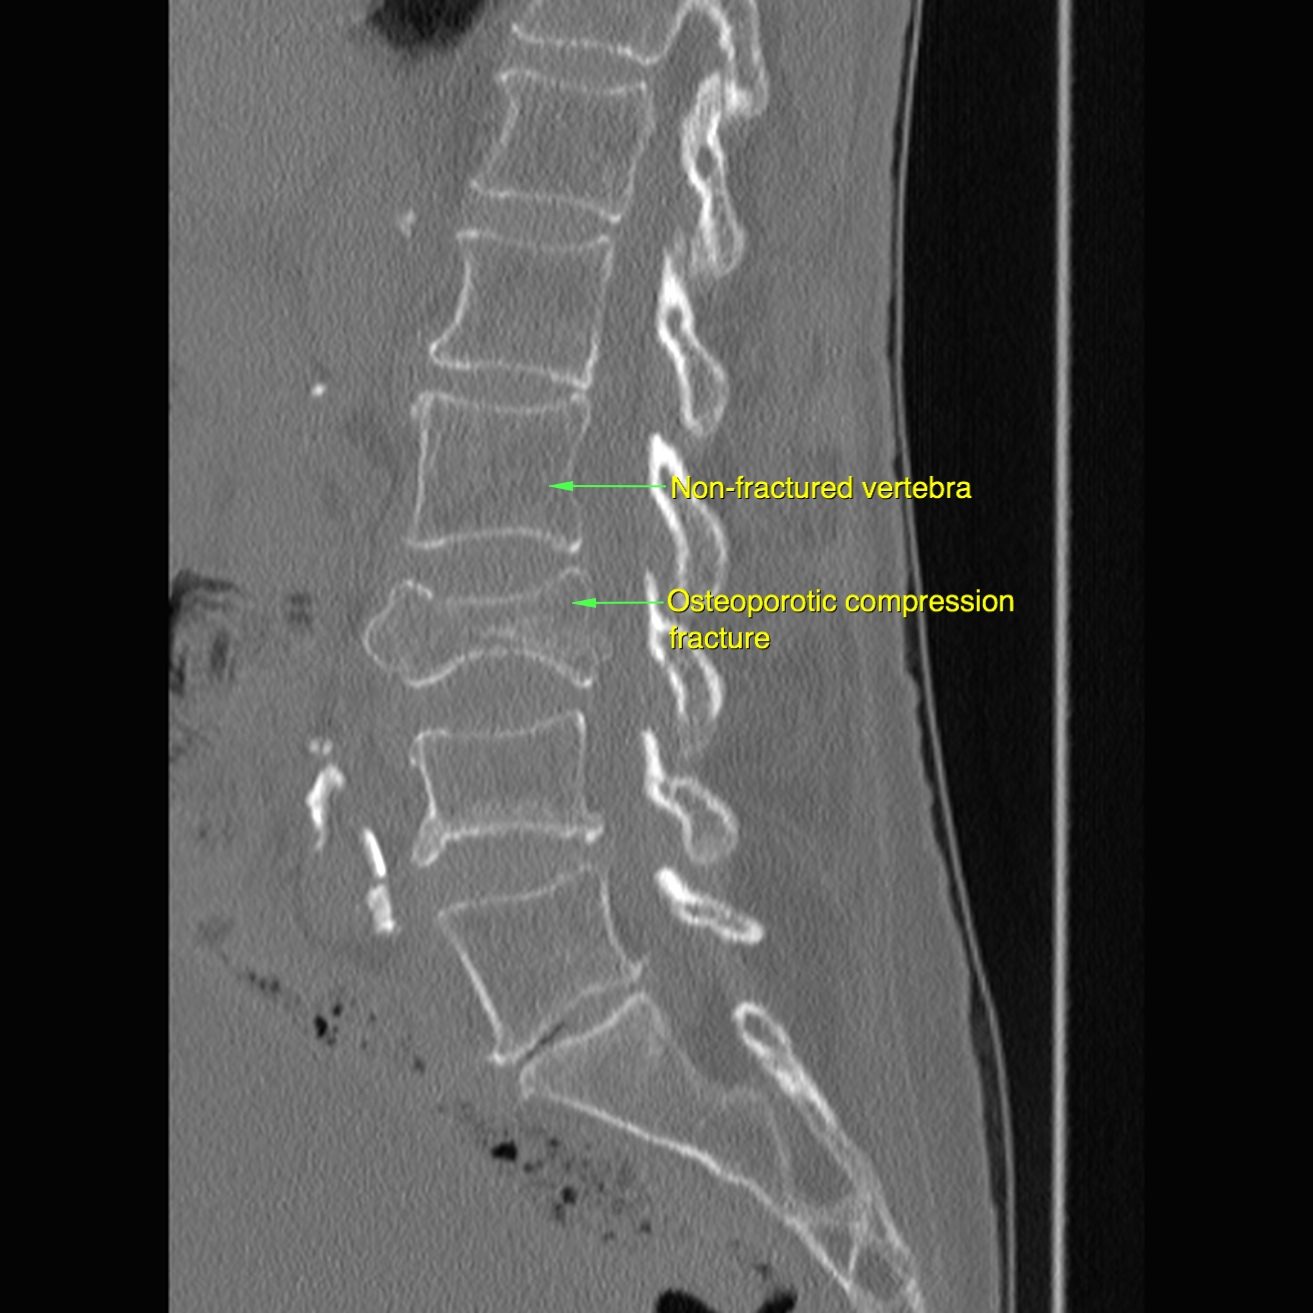
\includegraphics[width=1.0\textwidth,keepaspectratio]{media/compression-fx.jpg}
	\end{frame}
	\begin{frame}
	\frametitle{Attending Recommendation}
	\pause
	\centering
		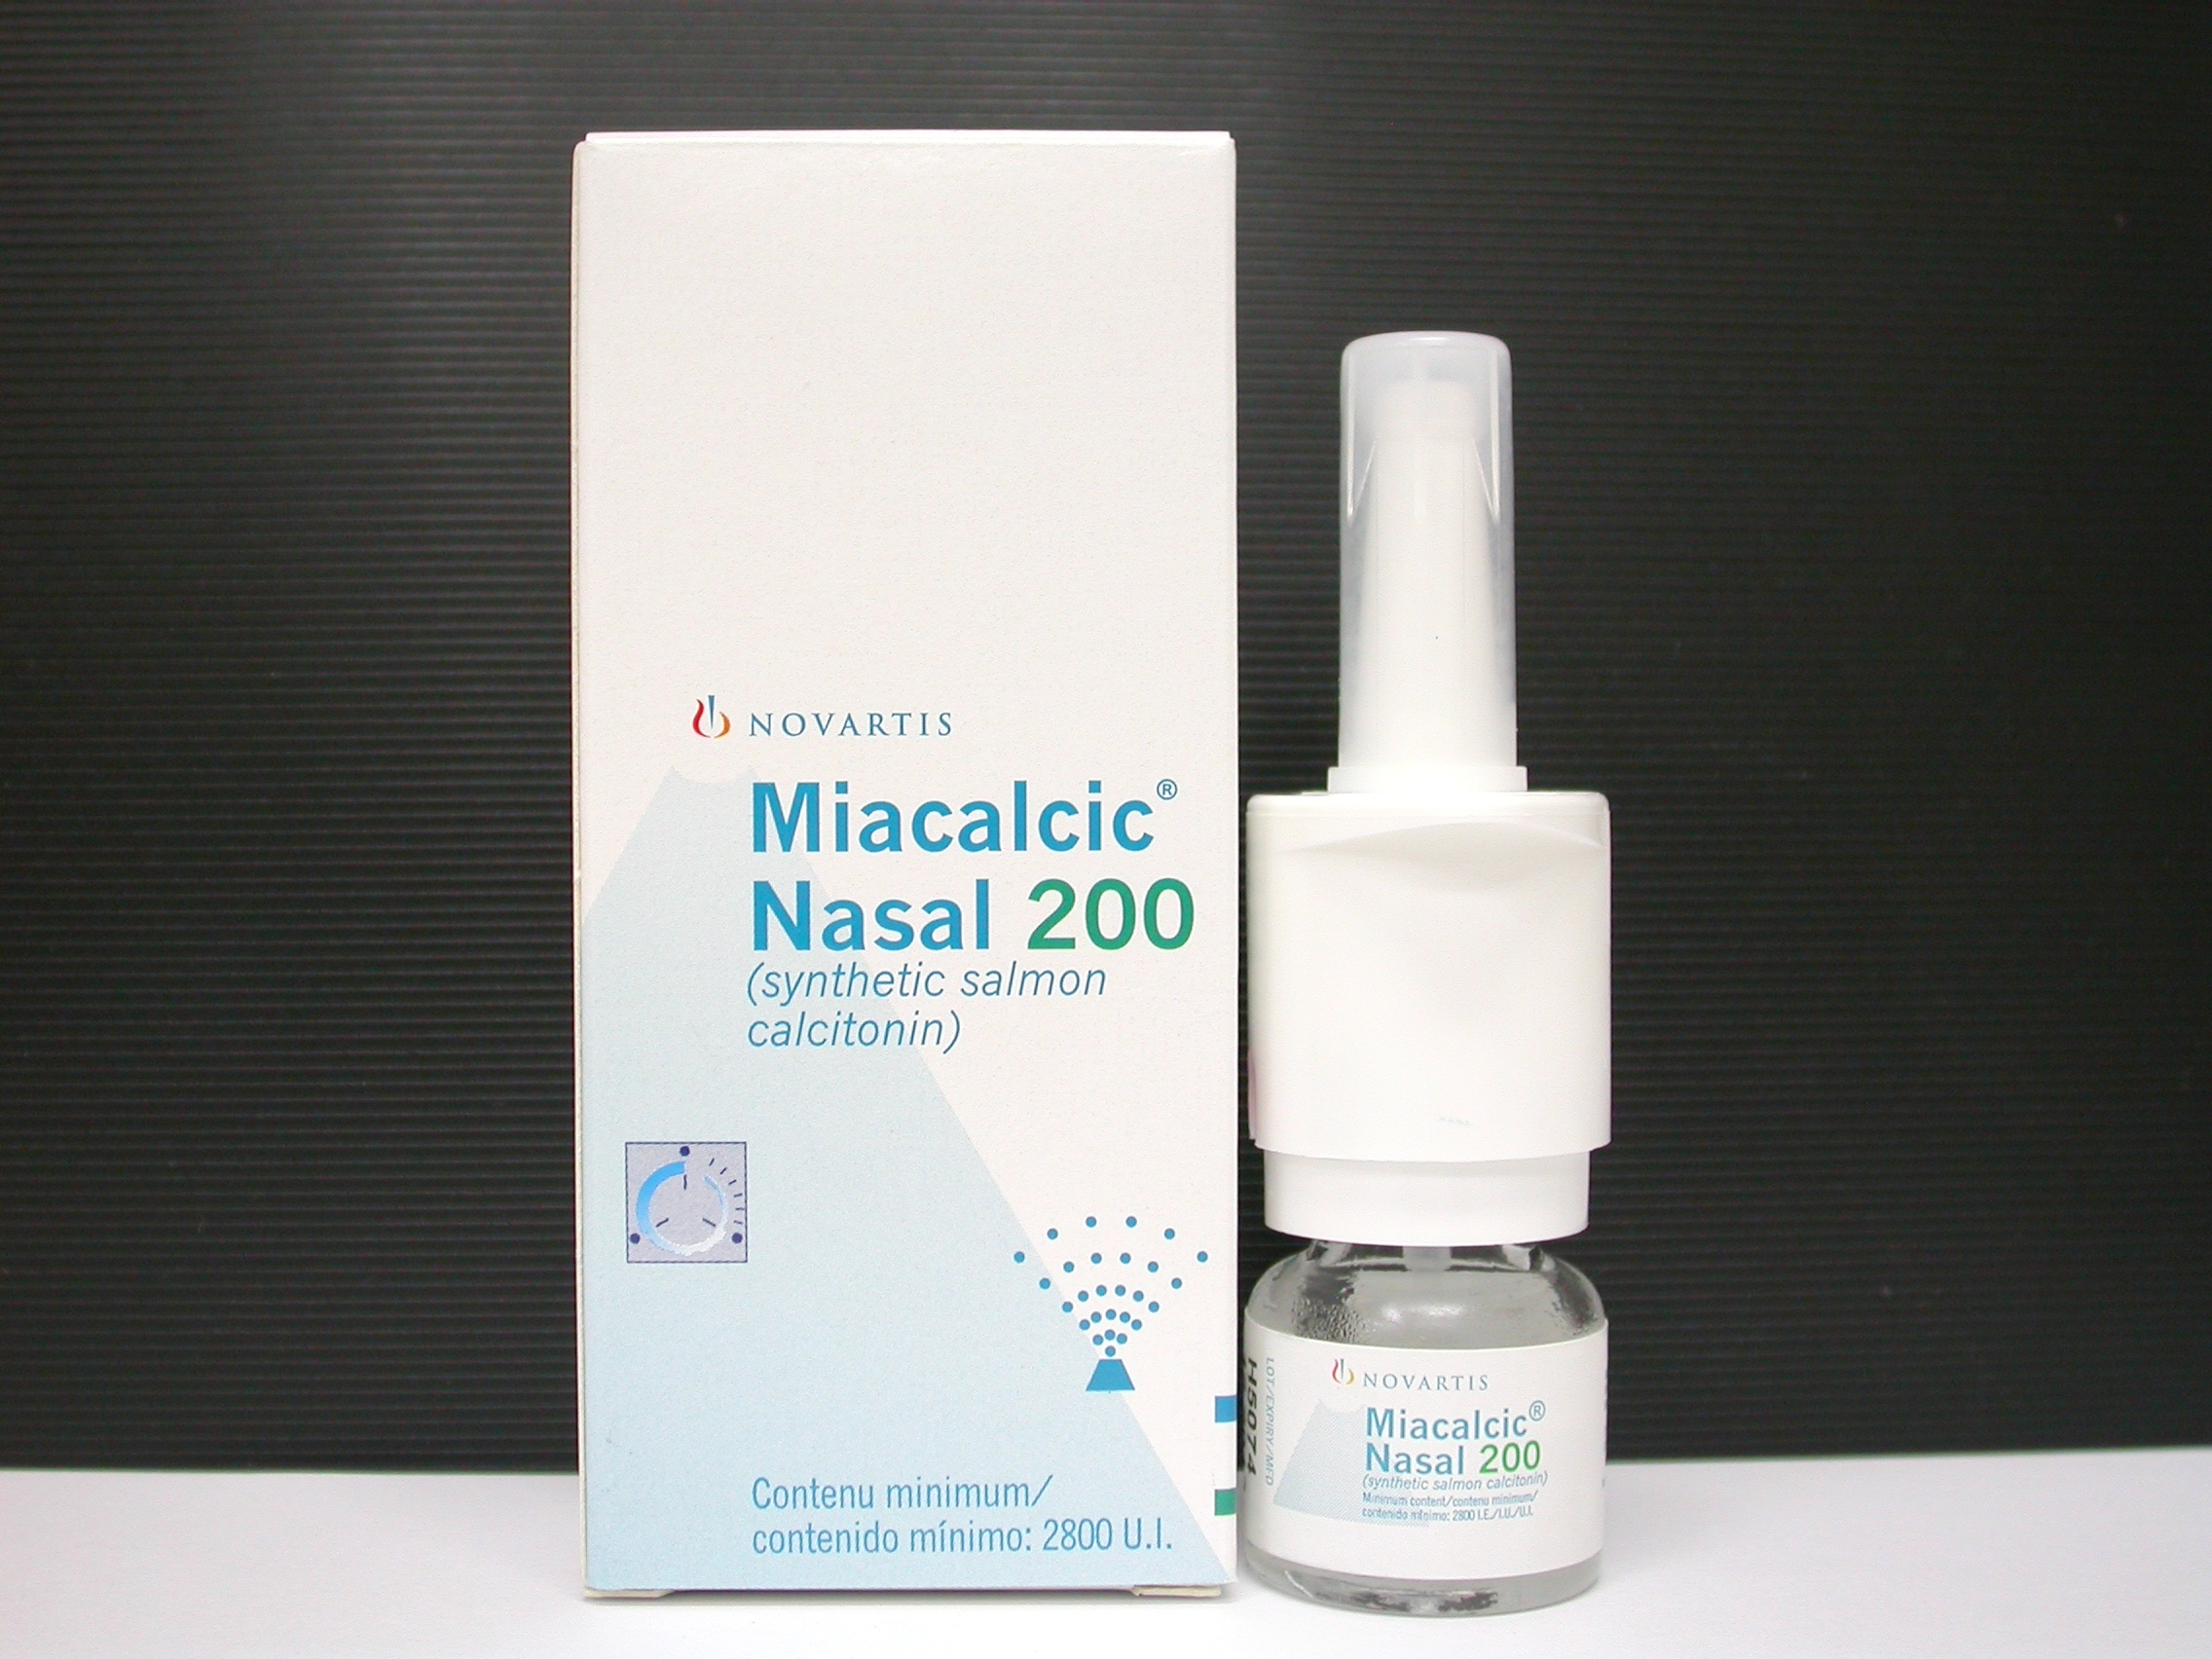
\includegraphics[height=0.9\textheight,keepaspectratio]{media/calcitonin-02.jpg}
	\end{frame}
\subsection{Research Question}
	\begin{frame}
	\frametitle{Research Question}
	\centering
	\begin{tabular}{l|l}
		\hline
		\textbf{Population} & adults $\geq$65 
		\\
		\hline
		\textbf{Intervention} & intranasal salmon calcitonin
		\\
		\hline
		\textbf{Comparison} & placebo
		\\ 
		\hline
		\textbf{Outcome} &  perceived pain at 1 week post-fracture
		\\
		\hline
	\end{tabular}
	\end{frame}
\section{Introduction}
\subsection{Risk, Incidence, and Definitions}
	\begin{frame}
		\frametitle{Risk and Incidence}
			\begin{itemize}
				\item in USA, 50-year-old woman has a 40\% lifetime chance of having a vertebral compression fracture\footfullcite{Tsuda2017} 
				\item risk factors
					\begin{itemize}
						\item low bone density
						\item age
						\item personal or family history of fracture, smoking, heavy drinking
						\item administration of steroids
						\item rheumatoid arthritis
					\end{itemize}
			\end{itemize}
	\end{frame}
	\begin{frame}
		\frametitle{Definition}
		\begin{columns}
			\column{0.5\textwidth}
			\centering
				\begin{itemize}
					\item Osteoporosis
						\begin{itemize}
							\item T-score $\leq-2.5$
						\end{itemize}
					\item Vertebral compression fracture
						\begin{itemize}
							\item a loss of $\geq$4  mm or 20\% of vertebral height
						\end{itemize}
				\end{itemize}
			\column{0.5\textwidth}
			\centering
			\pause
			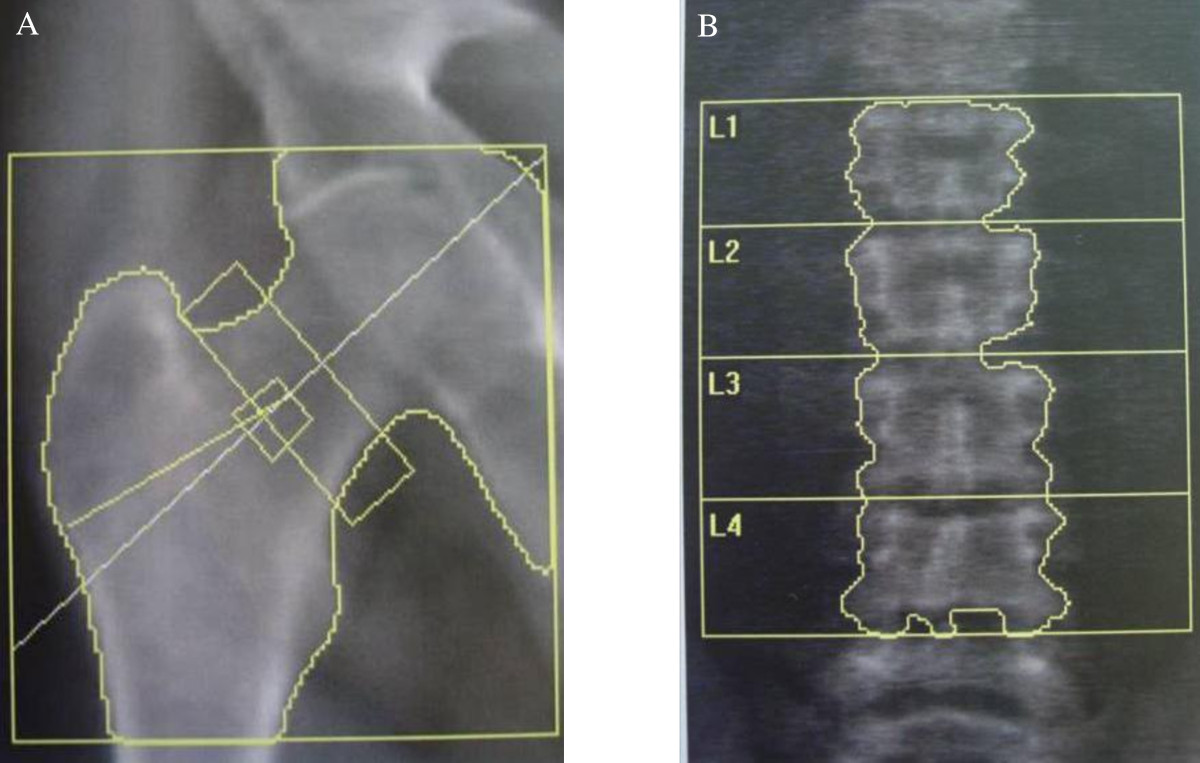
\includegraphics[width=0.9\textwidth,keepaspectratio]{media/dexa.jpg}
		\end{columns}
	\end{frame}
\section{Research Trial}
	\begin{frame}
		\frametitle{Lyritis et al. 2007}
			\begin{itemize}
				\item Several recent systemic reviews or meta-analyses show decreased pain at 1 and 4 weeks\footfullcite{Boucher2020}\footfullcite{Knopp-Sihota2012}.
				\item Most heavily rely on trials by Lyritis et al.
			\end{itemize}
	\end{frame}
\subsection{Study Design}
\begin{frame}
	\frametitle{Study Design}
	\begin{itemize}
		\item Population
		\begin{itemize}
			\item $n=100$, 32M \& 68F
			\item mean age 76 \& 71, respectively			
		\end{itemize}
		\item Inclusion Criteria
		\begin{itemize}
			\item Non-traumatic vertebral fracture w/in 5 days
			\item Radiograph-proven fracture
		\end{itemize}
	\item Intervention
		\begin{itemize}
			\item intra-nasal salmon calcitonin 200 U, 1 spray QHS
			\item intra-nasal NS, 1 spray QHS
		\end{itemize}
	\end{itemize}
\end{frame}
\subsection{Primary Outcomes}
\begin{frame}
	\frametitle{Primary Outcomes}
	\begin{itemize}
		\item  VAS pain score at 1 \& 4 weeks in multiple positions
		\begin{itemize}
			\item Bedridden
			\item Sitting
			\item Standing
			\item Walking
		\end{itemize}
	\end{itemize}
\end{frame}
\begin{frame}
	\frametitle{Primary Results}
		\centering
		\begin{tabular}{|l|l|l|l|}
			\hline
			\textbf{Group} & \textbf{Baseline} & \textbf{Week 1} & \textbf{Week 4}
			\\
			\hline
			bed, calcitonin & 9.0 & 4.9 & 1.0
			\\
			bed, placebo & 8.8 & 8.8 & 5.9
			\\
			\hline
			sit, calcitonin & 9.8 & 7.0 & 1.8
			\\
			sit, placebo & 9.6 & 9.5 & 6.8 
			\\
			\hline
			stand, calcitonin & 9.9 & 7.5 & 2.2
			\\
			stand, placebo & 9.9 & 9.9 & 8.7
			\\
			\hline
			walk, calcitonin & 10.0 & 9.1 & 3.1
			\\
			walk, placebo & 10.0 & 9.9 & 9.5
			\\
			\hline
		\end{tabular}
\end{frame}
\subsection{Secondary Outcomes}
\begin{frame}
	\frametitle{Secondary Outcomes}
	\textbf{Number of Bedridden Patients}
	\begin{center}
		\begin{tabular}{|c||c|c|c|c|c|}
			\hline
			Group & Baseline & Week 1 & Week 2 & Week 3 & Week 4
			\\
			\hline
			Calcitonin & 50 & 3 & 0 & 0 & 0
			\\
			\hline
			Placebo & 50 & 50 & 50 & 38 & 26
			\\
			\hline
			p value & -- & $<$0.0001 & $<$0.0001 & $<$0.0001 & $<$0.0001
			\\
			\hline
		\end{tabular}
	\pause
	\begin{itemize}
			\item Bone resorption
				\begin{itemize}
					\item hydroxyproline / creatinine ratio
					\item less bone resorption in calcitonin group
				\end{itemize}
	\end{itemize}
	\end{center}
\end{frame}
\subsection{Limitations}
\begin{frame}
	\frametitle{Limitations}
	\begin{itemize}
		\item Small sample ($n=100$)
		\item Problem of multiple testing
		\item Demographics and external validity
	\end{itemize}
\end{frame}
\subsection{Impact}
\begin{frame}
	\frametitle{Impact}
	\begin{itemize}
		\item First recommendation in AAOS guidelines\footfullcite{Esses2011}
		\begin{itemize}
			\item Quality of evidence, level II; strength moderate
		\end{itemize} 
		\item Recommend For
			\begin{itemize}
				\item ibandronate or strontium ranelate (QOE level I)
				\item L2 nerve root block (QOE level II)
				\item TLSO brace (inconclusive)
			\end{itemize}
		\item Recommend Against
			\begin{itemize}
				\item vertebroplasty or kyphoplasty
			\end{itemize}
	\end{itemize}
\end{frame}
\section{Conclusions}
\begin{frame}
	\frametitle{Conclusions}
	\begin{itemize}
		\item INSC viable option for osteoporotic vertebral fractures
		\item Few reported adverse effects
		\item Drug availability may limit use
		\item This patient's result
	\end{itemize}
\end{frame}
\section{References}
\begin{frame}
	\frametitle{References}
		\printbibliography
\end{frame}
\end{document}
